\documentclass[../main/main.tex]{subfiles}
\begin{document}

\chapter{Preliminaries}
\section{Quick review of Special Relativity}

Here we expose a quick review of Special Relativity in order to set the notations.\\


Fundamental principles of Special Relativity are followings:
\begin{enumerate}
\item All inertial reference frames are physically equivalent. There is no way to distinguish between different inertial frames in the sense that there is no preferred one. 
\item There exists universal (dimensional) constant: $c\simeq3\times10^8\text{m/s}$, i.e. the speed of massless particles.
\end{enumerate}


In order to implement these features basic ingredients are
\begin{enumerate}
\item Space and Time form a unique concept called \textbf{spacetime}. 
\item A spacetime is a collection of points called \textbf{event}.
\item Each inertial frame is associated with a set of \textbf{space time coordinates}. Each events is specified through coordinate system of a fixed initial frame. \[x^\mu=(x^0,x^1,x^2,x^3)\equiv(x^0,x^i)\equiv(ct,x,y,z)\equiv(ct,\vec x)\]
Usually $x,y,z$ are assumed to be Cartesian coordinates.


Given 2 events $A$ and $B$ in  spacetime 




\tikzset{every picture/.style={line width=0.75pt}} %set default line width to 0.75pt     
\[
\begin{tikzpicture}[x=0.75pt,y=0.75pt,yscale=-1,xscale=1]
%uncomment if require: \path (0,300); %set diagram left start at 0, and has height of 300

%Straight Lines [id:da9013720818372855] 
\draw    (195,224) -- (195,141) ;
\draw [shift={(195,139)}, rotate = 450] [color={rgb, 255:red, 0; green, 0; blue, 0 }  ][line width=0.75]    (10.93,-3.29) .. controls (6.95,-1.4) and (3.31,-0.3) .. (0,0) .. controls (3.31,0.3) and (6.95,1.4) .. (10.93,3.29)   ;
%Straight Lines [id:da7261382621997787] 
\draw    (195,224) -- (302.5,224) ;
\draw [shift={(304.5,224)}, rotate = 180] [color={rgb, 255:red, 0; green, 0; blue, 0 }  ][line width=0.75]    (10.93,-3.29) .. controls (6.95,-1.4) and (3.31,-0.3) .. (0,0) .. controls (3.31,0.3) and (6.95,1.4) .. (10.93,3.29)   ;
%Straight Lines [id:da22577623387415535] 
\draw    (195,224) -- (141.99,271.66) ;
\draw [shift={(140.5,273)}, rotate = 318.03999999999996] [color={rgb, 255:red, 0; green, 0; blue, 0 }  ][line width=0.75]    (10.93,-3.29) .. controls (6.95,-1.4) and (3.31,-0.3) .. (0,0) .. controls (3.31,0.3) and (6.95,1.4) .. (10.93,3.29)   ;
%Straight Lines [id:da04380450147553239] 
\draw [color={rgb, 255:red, 65; green, 117; blue, 5 }  ,draw opacity=1 ][line width=0.75]    (219.5,203) -- (276.5,169) ;
\draw [shift={(276.5,169)}, rotate = 329.18] [color={rgb, 255:red, 65; green, 117; blue, 5 }  ,draw opacity=1 ][fill={rgb, 255:red, 65; green, 117; blue, 5 }  ,fill opacity=1 ][line width=0.75]      (0, 0) circle [x radius= 1.9, y radius= 1.9]   ;
\draw [shift={(219.5,203)}, rotate = 329.18] [color={rgb, 255:red, 65; green, 117; blue, 5 }  ,draw opacity=1 ][fill={rgb, 255:red, 65; green, 117; blue, 5 }  ,fill opacity=1 ][line width=0.75]      (0, 0) circle [x radius= 1.5, y radius= 1.5]   ;

% Text Node
\draw (120,137) node    {$$};
% Text Node
\draw (283,258) node    {$x,y,z$};
% Text Node
\draw (177,141) node    {$ct$};
% Text Node
\draw (210,207) node    {$A$};
% Text Node
\draw (280,157) node    {$B$};


\end{tikzpicture}\]

their distance is $\Delta x^\mu=x^\mu_B-x_A^\mu$. We introduce the (squared) \textbf{Minkowski distance}
\[\Delta s^2=\eta_{\mu\nu}\Delta x^\mu\Delta^\nu\quad\text{where}\quad\eta_{\mu\nu}=\begin{pmatrix}-1&&&\\&1&&\\&&1&\\&&&1\end{pmatrix}\]
where $\eta_{\mu\nu}$ is \textbf{Minkowski metric}.
This induces the \textbf{line element}
\[\de s^2=\eta_{\mu\nu}\de x^\mu\de x^\nu\]
This element is scalar quantity and therefore does not depends on the specific inertial frame.

The quantity $\Delta s^2$ has an intrinsic meaning
\[\begin{cases}\begin{alignedat}{2}
&\Delta s^2>0\quad&&:\quad \Delta x^\mu\text{ is \textbf{space-like} vector}\\
&\Delta s^2=0\quad&&:\quad \Delta x^\mu\text{ is \textbf{time-like} vector}\\
&\Delta s^2<0\quad&&:\quad \Delta x^\mu\text{ is \textbf{light-like/null} vector}
\end{alignedat}\end{cases}\]
Space-like vector means that exists different frames were two events are simultaneous. Time-like vector means that exists different frames where two events have same space coordinates but they happen at different times. Light-like vectors means that two events may be connected by a light signal.

\item Allowed transformations for spacetime vectors must preserve the line element: $\Delta\tilde s^2=\Delta s^2$. These transformations are the \textbf{Poincaré Transformations}

\[x^\mu\quad\to\quad\tilde x^\mu={\Lambda^\mu}_\nu x^\nu+a^\mu\qquad\text{with}\qquad{\Lambda^\rho}_\mu{\Lambda^\sigma}_\nu\eta_{\rho\sigma}=\eta_{\mu\nu}\]


\end{enumerate}

\skipline
Once we have reformulated notions of space and time, we have to reformulate law of physics in such a way they does not depends on the reference frame.

Trajectories of point like-particles are associated to curved \textbf{wordlines} in space time and described evolution of events. Mathematically they are described by maps from $\RR$ into a set of four functions: $\lambda\in\RR\to x^\mu(\lambda)$. Near if we consider nearby events separated by infinitesimal shift we can obtain infinitesimal variation of coordinates:
\[\de x^\mu(\lambda)\equiv x^\mu(\lambda+\de\lambda)-x^\mu(\lambda)=\frac{\de x^\mu(\lambda)}{\de\lambda}\de\lambda\]
Since no particles can move at a speed higher then light this implies that $\de s^2$ must be time-like. Notice that choice of parameter $\lambda$ is free. One possible choice of this parameter is the \textbf{(differential) proper time}:
\begin{align*}
\de\tau\equiv\sqrt{-\de s^2}
&=\de\lambda\sqrt{-\eta_{\mu\nu}\dot x^\mu(\lambda)\dot x^\nu(\lambda)}
=c\,\de t\sqrt{1-\frac{v^2}{c^2}}\equiv\frac{c\,\de t}\gamma
\end{align*}
where third step holds if $\lambda\equiv t$. If we define $\beta\equiv v/c$ \footnote{This is the speed in natural units, i.e. in units of $\beta$. If we set $c=1$ then $v=\beta$.}, then $\gamma=1/\sqrt{1-\beta^2}$ is called \textbf{Lorentz factor}. Notice that last step implies time dilatation at higher velocities. For $\lambda=t$ we obtain
\[\tau=c\int\de t\sqrt{1-\frac{v^2}{c^2}}\]
i.e. with this definition the proper time has dimension of a length $[\tau]=L$. Physically the proper times it's the time measured by a clock moving along the trajectory. 

Proper time allow us to define a vector called \textbf{4-velocity} that can be identified as relativistig generalization of velocity. Namely:
\[u^\mu(\tau)=\frac{\de x^\mu(\tau)}{\de\tau}=\left(\gamma,\gamma\frac{\vec v}{c}\right)\]
Notice 
\[u^\mu u_\mu=-1\]
i.e. is a time-like vector. Moreover, this vector has only three degrees of freedom, since one component is fixed by previous propriety.


Now we can define the generalization of acceleration, \textbf{4-acceleration}, as follows
\[\alpha^\mu(\tau)=\frac{\de u^\mu(\tau)}{\de \tau}\]
Notice that, as we expected, 4-acceleration is orthogonal to 4-velocity
\[u_\mu\alpha^\mu=0\]
and this implies that $\alpha^\mu$ is a space-like since it is orthogonal to a time-like vector.

This proves a relativistic generalization of distance, speed and acceleration. Also laws of dynamic can be generalizated, in particular if we define the \textbf{four-force} $f^\mu$ as the generalization of force we can obtain the
 \textbf{Relativistic Second Newton's law}:
\[mc\alpha^\mu\equiv\frac{\de p^\mu}{\de\tau}=f^\mu\]
where we used four acceleration or equivalently the generalization of newtonian momentum, \textbf{4-momentum},
\[p^\mu\equiv mcu^\mu=\p{\frac Ec,\vec p}\]

For example, for Lorentz force
\[\vec F_L=e\p{\vec E+\frac1c\vec v\cross\vec B}\]
can be generalizzated in a manifestly covariant way into\footnote{Here is evident that this formula does not change under Poincaré transformations.}
\[f^\mu_L=\frac ecF^{\mu\nu}u_\nu\hspace{1.5cm}\text{with}\quad F^{\mu\nu}=
\begin{pmatrix}0&E_1&E_2&E_3\\-E_1&0&B_3&-B_2\\-E_2&-B_3&0&B_1\\-E_3&B_2&-B_1&0\end{pmatrix}\]
where $F^{\mu\nu}$ is the \textbf{EM-Tensor}.

We can also rewrite Maxwell equations into two covariant equation
\[\partial_\mu F^{\mu\nu}=-\frac{4\pi}{c}j^\nu\quad,\quad\partial_{[\mu}F_{\nu\rho]}=0\]
where the former, inhomogeneous, shows the \textbf{4-current} $j^\mu=(c\rho, \vec j)$. The second equation, homogeneous, exhibits total antisymmetrized indexes\footnote{$\partial_{[\mu}F_{\nu\rho]}=\partial_{\mu}F_{\nu\rho}+\partial_\rho F_{\mu\nu}+\partial_\nu F_{\rho\mu}$.}. Each of these equations contains 2 independent equations.


We can conclude saying that all possible interactions can be written in a covariant way, except from gravitation. In order to include this force General Relativity has been developed.


%%%%%%%%%%%%%%%%%%%%%%%%%%%%%%%%%%%


\section{Relativity and Gravitation}

Before Einstein formulated General Relativity the accepted theory for Gravity was Newton's one.

In Newton theories particles interact according to \textbf{Newton's universal gravity law}:
\[\vec F_G=-\frac{GmM}{\vert\Delta\vec r\vert^3}\Delta\vec r\qquad G\simeq6.67\times10^{-11} \frac{m^3}{kg\cdot s^2} \]
where $\vec F_G$ is the (always) attractive gravitational force, $\Delta\vec r$ is the distance (at same time) between particles, and $G$ is \textbf{Newton's gravitational constant}.

The point is that this law is not invariant under Poincaré. Practically this is evident since positions are evaluated at a certain time and therefore when a particle moves the corresponding formula for gravitational force changes instantaneously. This is unphysical since physical signal cannot travel with a velocity higher than  speed of light. This instantaneous interaction between particles cannot be compatible with special relativity.

One possible strategy to way out is to look at an analogy with Coulomb force between two particles $A$ and $B$:
\[\vec F_C=e_B\vec E=\frac{e_Be_A}{\vert\Delta\vec r\vert^3}\Delta\vec r\]
These formulas are very analogous. The coulomb force is valid only in a static setting in which one put one particle in the electric field of the other. When particles moves this particles does not hold anymore since we have to consider magnetic field and Coulomb force must be substituted with the more general Lorentz force.


Let's go further with the analogy. In gravity we can introduce a potential which is completely analogous to electric static potential:
\begin{align*}
\nabla^2\Phi=4\pi G\rho_M\hspace{2cm}G\rho_M\leftrightarrow&-\rho_{el}\hspace{2cm}\nabla^2\Phi_{el}=-\vect\nabla\cdot\vec E=-4\pi\rho_{el}\\
\vec F_G=-m\vect\nabla\Phi\hspace{2.8cm}m\leftrightarrow&e\hspace{3.2cm}\vec F_C=e\vec E=-e\vect\nabla\Phi_{el}
\end{align*}
where $\Phi$ describe potentials and $\rho$ describes distributions. 

In order to make Coulomb force compatible with special relativity we have to consider EM theory in a wider way, in order to express quantities in tensorial way:
\begin{alignat*}{2}
&\Phi_{el}\hspace{1cm}&&\rightarrow\quad	A^\mu=(\Phi, \vec A)\\
&\vec E\hspace{1cm}&&\rightarrow\quad	F_{\mu\nu}=\partial_\mu A_\nu-\partial_\nu A_\mu\\
&\rho_{el}\hspace{1cm}&&\rightarrow\quad	j^\mu=(c\rho_{el},\vec j)\\
m\vec a&=\vec F_c\hspace{1cm}&&\rightarrow\quad	mc\alpha^\mu=f^\mu_L=\frac ecF^{\mu\nu}u_\nu
\end{alignat*}
So in order to understand how to make gravity compatible with spacial relativity we should find gravitational analogous to previous completions of Coulomb theory. We will start from the last  step, i.e. we have to understand what happen when we put a particle in an external gravitational field and then derive covariant relations, which in non relativistic approximation must leads to Newton's law
\[m\vec a=\vec F_G\]
In particular we have to find which is relativistic generalization of gravitational field $\Phi_G$ that allows us to build a covariant theory of gravitation.

\skipline
First of all we have to highlight a deep difference between $\vec F_G$ and $\vec F_C$ that in principle we should distinguish between two forces. For gravitational theory the force is proportional to the mass of the particle, while for Coulomb law the force is proportional to the charge. In order to make the analogy precise we have should distinguish between two different concepts of mass, that in principle may be differnet\footnote{For the moment we consider the non-relativistic limit}
\begin{alignat*}{2}
&\text{\textbf{interial mass }} m_I\quad&&:\quad m_I\vec a=\vec F_G\\
&\text{\textbf{gravitational mass }} m_G\quad&&:\quad\vec F_G=-m_G\vect\nabla\cdot\Phi\hspace{1cm}m_G\sim\text{gravitational charge}
\end{alignat*}
the fact that in Newton's law $m_G\equiv m_I$ is an highly not-obvious feature from theoretical point of view. Indeed, this is the Newtonian manifestation of the \textbf{(Weak) Equivalence principle}.

\subsection{The Equivalence principle}

The Equivalence principle is the consequence of the central observation that $m_G\equiv m_I$. This implies that
\[\slashed m_I\vec a=\vec F_G=-\slashed m_G\vect\nabla\Phi\quad\Rightarrow\quad\boxed{\vec a=-\vect\nabla\Phi}\]
i.e. acceleration of a mass is the same for each value of $m$ (for example this does not happen for Coulomb interaction, where acceleration depends on the charge of the particle). Then for the same field $\Phi$ all bodies fall with the same acceleration. 

This is a very important observation: if $\vect\nabla\Phi$ is considered approximatively constant in a chosen frame, then we cannot distinguish between gravitational force and an apparent force due to an acceleration in the opposite direction of this frame with respect to an inertial frame. 


\begin{figure}[H]
\centering
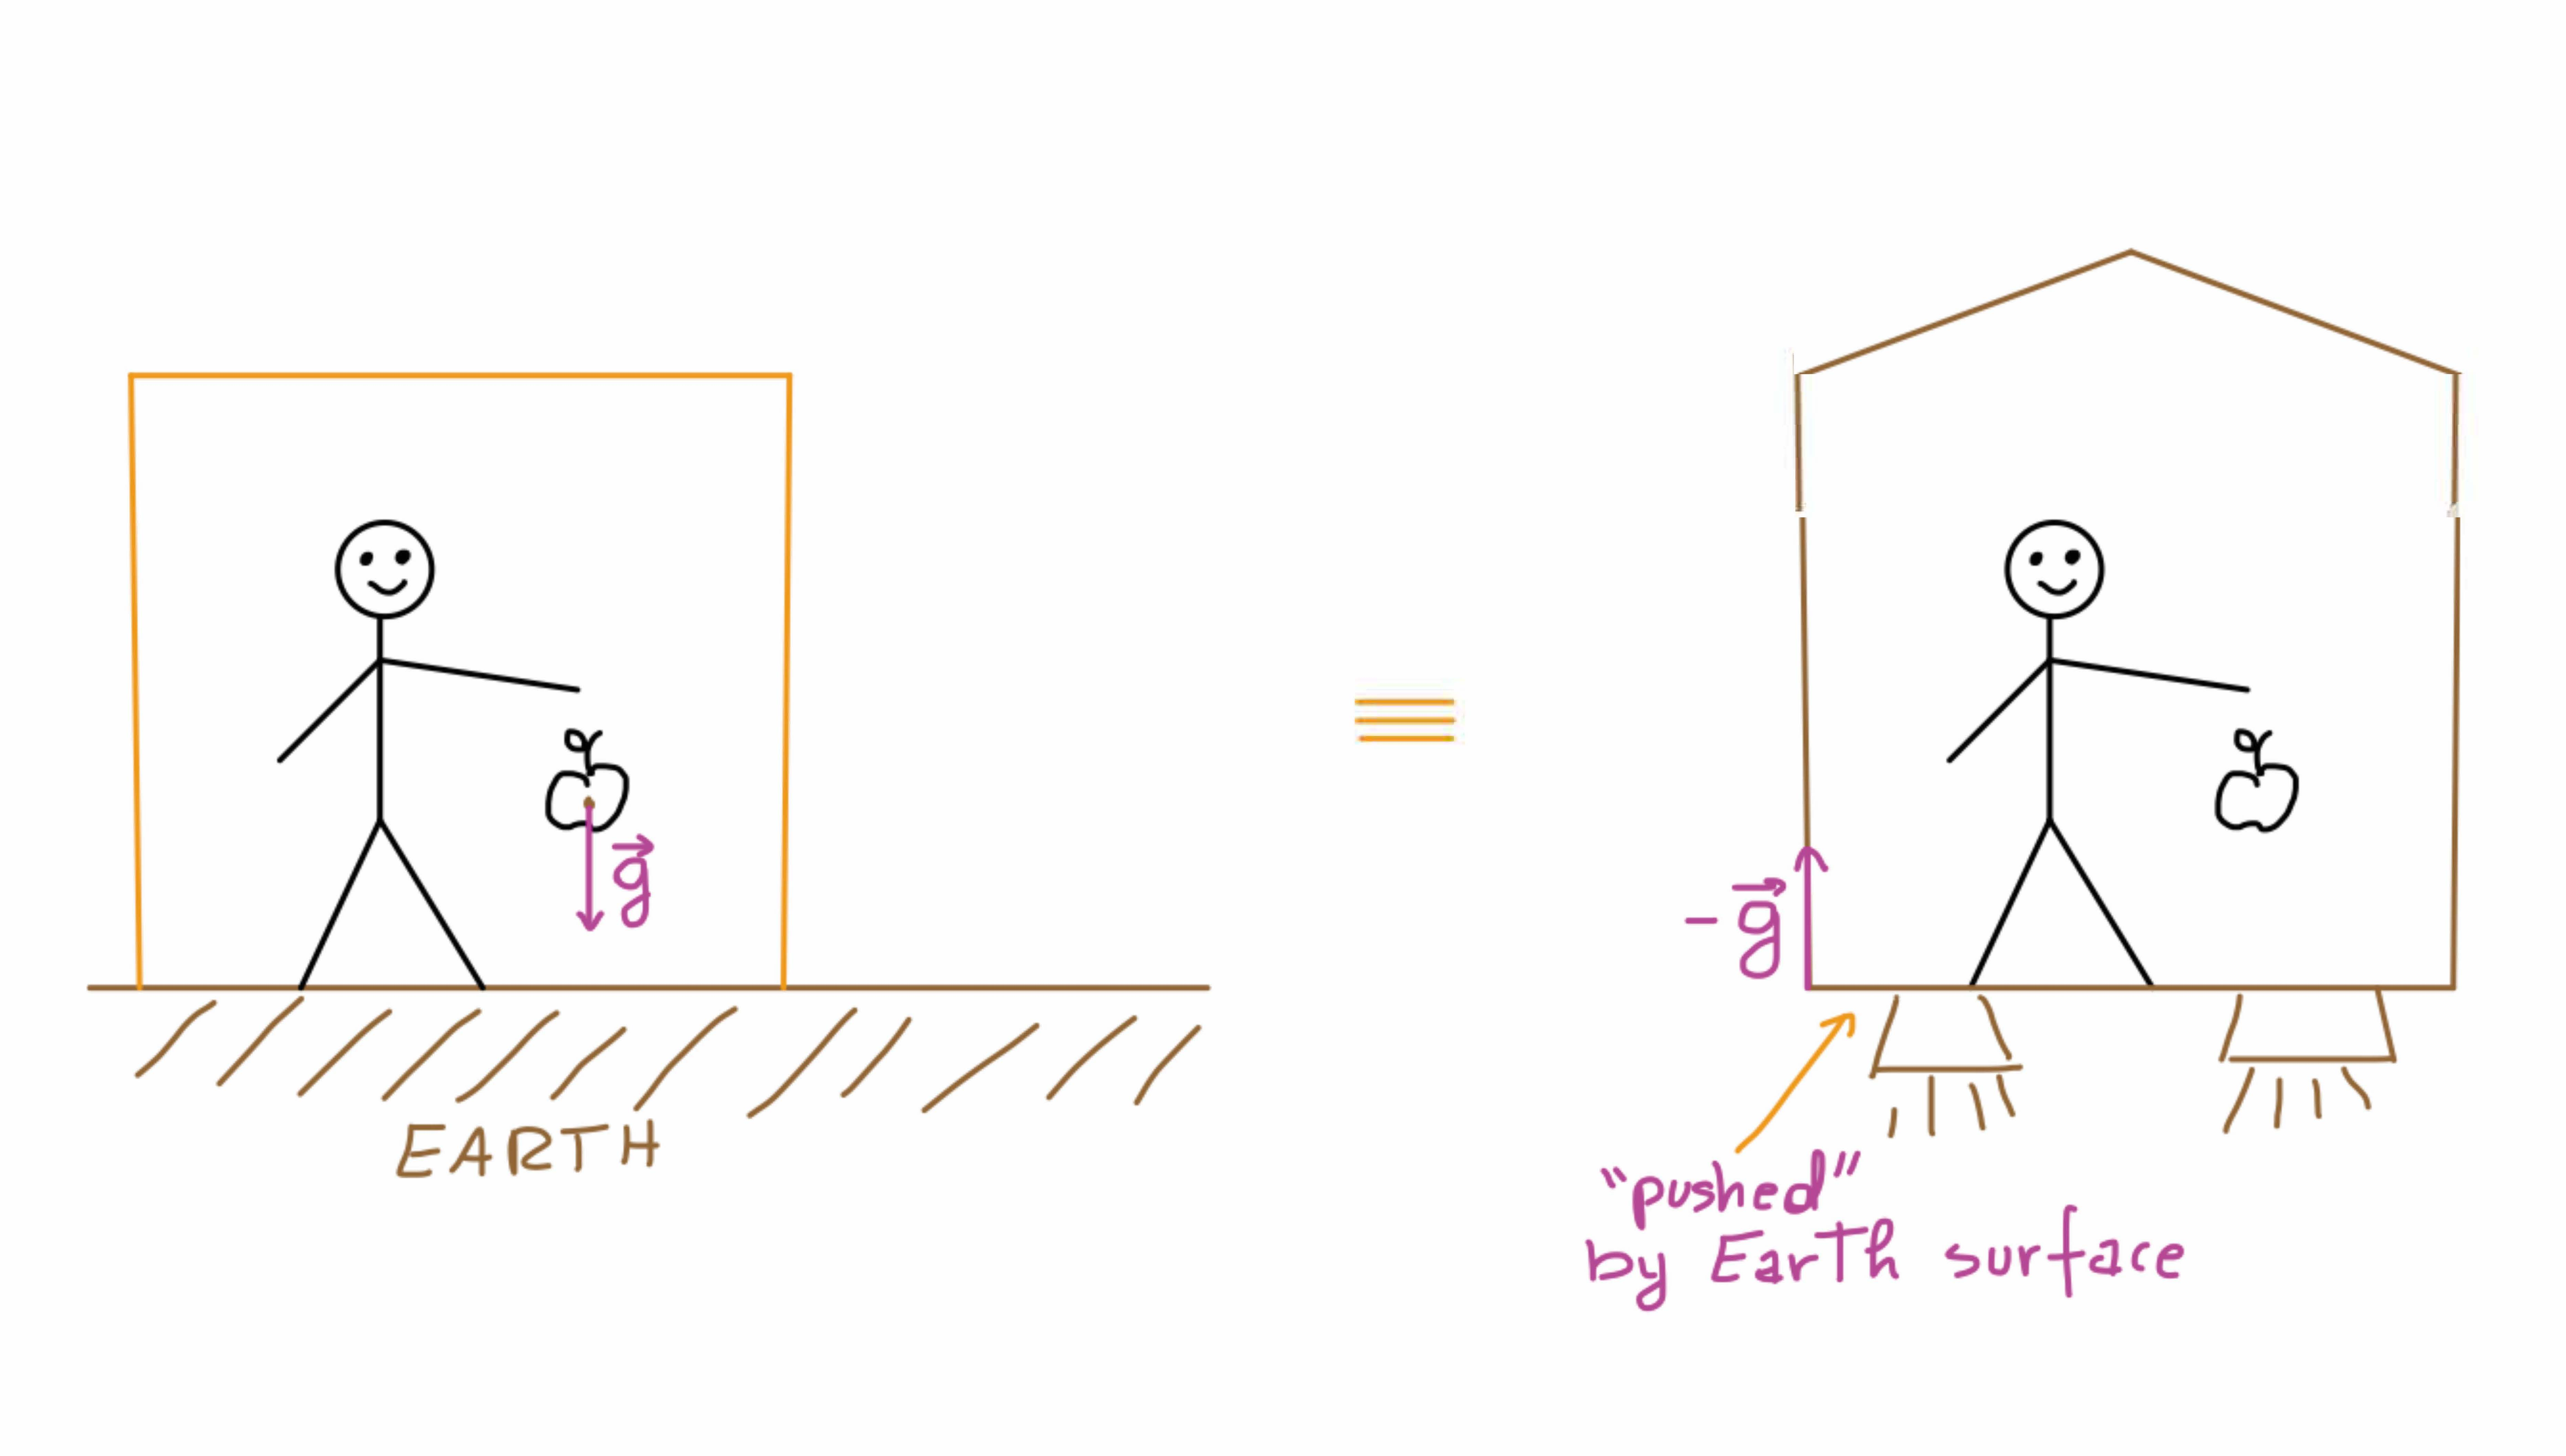
\includegraphics[width=11cm]{../img/equivalence-principle.jpg}
\caption{In the first figure the apple falls down, while in the second the rocket moves upward. Our Rocket Man can't fell any difference.}
\end{figure}

\subsubsection{``The happiest thought of Einstein life'':}
\begin{mdframed}[style=mybox]
``The gravitational field has only a \emph{relative} existence $\dots$ because for an observer freely falling from the roof of a house there exists - at least in the immediate surroundings - no gravitation''
\end{mdframed}

In other words, a freely falling system can be identified (up to some approximations) to an ``inertial'' frame\footnote{We will have to specify this concept in formalization of General Relativity.} in the sense that within a freely falling system there is no way to distinguish between these two situations. 

This leads to the formulation of \textbf{(Einstein) Equivalence ``Principle''} (\textbf{EEP})
\begin{mdframed}[style=mybox]
In a small enough region of spacetime, the laws of physics reduce to those of Special Relativity: it is impossible to detect the existence of a gravitational field by means of local experiments.
\end{mdframed}

In other words though local experiments it is impossible to distinguish between a system accelerated and a system subjected to gravitational field.
The caveat ``small enough'' refers to the \emph{Tidal effects}, i.e. the previous statement holds only if the gravitational field can be considerated uniform and constant. Let $l$ be the typical length scale of our experiment and $L$ be the distance from the mass that origins the gravitational field, then ``small enough'' means
\[\p{\frac lL}^n\ll1\]

\begin{figure}[H]
\centering
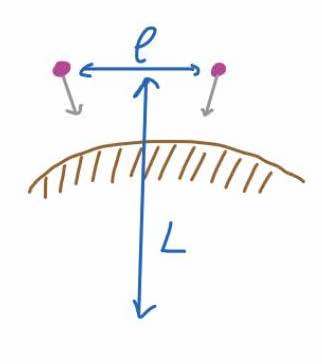
\includegraphics[width=4cm]{../img/Tidal-effect.jpg}
\caption{Tidal effect}
\end{figure}

There are 3 kinds of equivalence principles:\footnote{In the paper \emph{Di Casola, Liberati \& Sonego}, 1310.7426, are described differences of these statements and experiments evidence for each principle.}
\begin{enumerate}
\item\textbf{Weak Equivalence Principle (WEP)}: regards only experiments on freely falling non back-reacting test particles (direct consequence of $m_G=m_I$.
\item\textbf{Einstein Equivalence Principle (EEP)}: previously stated, include also other non-gravitational local experiments (no backreaction)
\item\textbf{Strong Equivalence Principle (SEP)}: includes also local gravitational effects (includes gravitational effects, i.e. back-reaction). For instance it consider also inertial masses in experiments involving them variation measure when accelerated. 
\end{enumerate}

One can think about these principles as heuristic ideas, which will be defined in a more precise way by General Relativity in a concrete framework. 


There are some immediate implications of these principles. First \emph{light is deflected} in presence of gravitation potential, this is obvious watching at the next image


\begin{figure}[H]
\centering
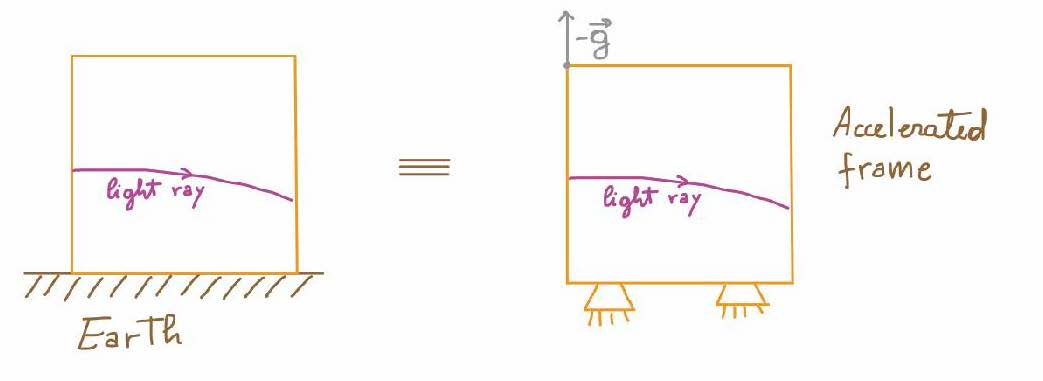
\includegraphics[width=11cm]{../img/light-deflection.jpg}
\end{figure}

Then, we will see \emph{gravitational time dilatation and red-shift of light}:

\begin{figure}[H]
\centering
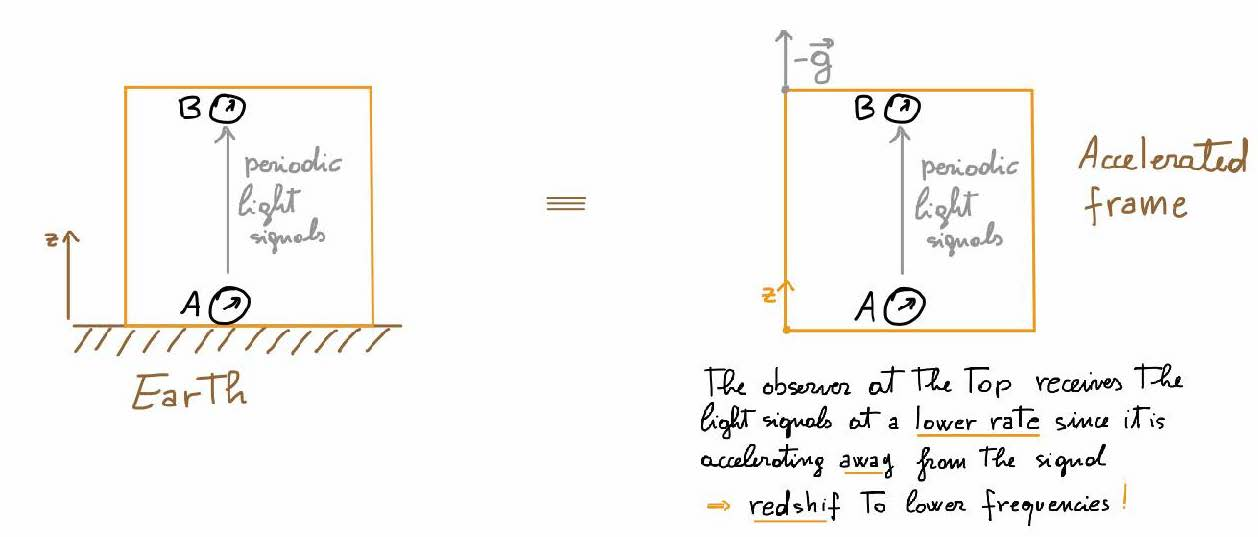
\includegraphics[width=11.5cm]{../img/redshift.jpg}
\end{figure}

The second frame is accelerated, then during the interval which the light signal need to go from a clock A to the clock B the clock B gets some additional velocity, so frequency measured by B is lower than the frequency measured by A:
\[v_B-v_a\simeq g\Delta t=g\frac{\Delta z}{c}\]
and we can observe a \emph{Doppler effect} 
\[\frac{\nu_B-\nu_A}{\nu_a}\simeq\frac{v_A-v_B}{c}=\frac{g(z_A-z_B)}{c^2}\]
If we take $\Phi\simeq gz$ we can obtain an explicit relation between redshift and acceleration
\[\frac{\nu_B-\nu_A}{\nu_A}\simeq\frac1{c^2}(\Phi_A-\Phi_B)<0\]
Viceversa, since frequency is the inverse of time interval, this can be interpreted as a time dilatation.
In other words, we can see that clock B ``sees'' clock A moving more slowly.\footnote{See Hartle's book for the discussion of Redshift using time dilatation instead of moving clocks.}



\section{The constantly accelerated elevator}
\textbf{Blau sec. 1.3; 't Hooft chap. 3}\\

Now we have to make more concrete what we introduced in the previous chapter, i.e. we want to extend in a covariant way the gravitational potential, using the equivalence principle. Up to the present, we obtained the equivalence principle using non-relativistic arguments, now we want to obtain same result using a suitable mathematical framework, which allows us to derive gravitational laws in a covariant way. 

From now on we will use relativistic units for velocity, i.e. all velocities are expressed in units of $c$. This is the same as set $c=1$. With this choice
\[[L]=[T]\,,\qquad [E]=[M]\,,\,\quad\dots\]

Now we have to look for a natural frame with its own natural coordinates which describe uniform accelerated frame. Recall that in SR a trajectory with constant acceleration will not make physical sense because any particle undergoing constant acceleration at a certain time would exceedes the speed of light, leading to a non-physical propagating signal. 

On the other hand a proper definition of a uniformly accelerating trajectory is to impose that the proper acceleration is constant. For example for a rocket travelling with a constant proper acceleration $a$ along $ x$:
\[\alpha^\mu\alpha_\mu=a^2\qquad\text{with}\quad \alpha^\mu=(\alpha^0,\alpha^1,0,0)=\frac{\de u^\mu}{\de\tau}\]
The interpretation of this proper acceleration is that this is exactly the acceleration measured in the instantaneous rest-frame of the rocket. This means that when we consider the trajectory of the rocket we should think about a specific point of the rocket. Then this point will accelerate, but in any instant of time we can choose a rest frame $S_I$ where the four velocity takes the form
\[u^\mu\vert_{S_I}=(1,0,0,0)\]
and since $\alpha^\mu u_\mu=0$ we have
\[\alpha^\mu|_{S_I}=(0,a,0,0)\]
where $a$ is constant during the acceleration. 
%
Then we can explicitly write down the form of a trajectory that satisfies this relation in the following form
\begin{equation}\label{eqn:const-accell-solut}\begin{cases}\begin{alignedat}{4}
&t(\tau)&&=x^0(\tau)&&=\frac1a\sinh(a\tau)&&=X\sinh(\frac\tau X)\\
&x(\tau)&&=x^1(\tau)&&=\frac1a\cosh(a\tau)&&=X\cosh(\frac\tau X)
\end{alignedat}\end{cases}\end{equation}
where $X\equiv1/a$. Notice that $(x^0,x^1)(0)=(0,X)$, as it's shown in the next figure:

\begin{figure}[H]
\centering
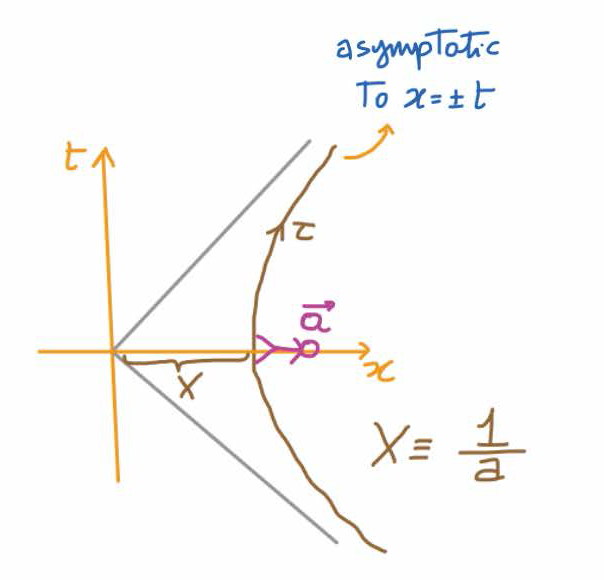
\includegraphics[width=5cm]{../img/const-accel-traject.jpg}
\caption{The green line describe the trajectory, parametrized by $\tau$. In the picture are represented only first two coordinates.}
\end{figure}

A the notation suggests the parameter $\tau$ is the proper time, indeed we can check it computing $\de s^2$ over the trajectory:
\[\de s^2=-\de t^2+\de x^2=-\cosh^2(a\tau)\de \tau^2+\sinh^2(a\tau)\de\tau^2=-\de\tau^2\]
this implies
\[\int_0^\tau\sqrt{-\de s^2}=\int_0^\tau\de\tilde\tau=\tau\]
i.e. $\tau$ is exactly the proper time. 
It is also immediate to check that these trajectories satisfies our requirement
\[\begin{cases}
u^0(\tau)=\cosh(a\tau)\\
u^1(\tau)=\sinh(a\tau)
\end{cases}
\qquad
\Rightarrow
\qquad
\begin{cases}
\alpha^0(\tau)=a\sinh(a\tau)\\
\alpha^1(\tau)=a\cosh(a\tau)
\end{cases}
\qquad
\Rightarrow
\qquad
\alpha^\mu\alpha_\mu=a^2
\]
In order to simplify the notation in the following we will use also the (well known from SR) relation: $\gamma=\cosh(\tau/X)$.

Notice also that eq.\eqref{eqn:const-accell-solut} is a particular solution that satisfies the requirement of constant acceleration. We fixed integration constants so that any trajectory of this form asymptotically tends to the straight line $t=\pm x$ that describes the light-like signal passing through the origin. With this specific choice $X=1/a$ can be identified with the $x$-position at $t=\tau=0$.

Letting $X=1/a$ change we get a family of hyperbolic trajectories 
\[x^2-t^2=X^2\equiv1/a^2\]

\begin{figure}[H]
\centering
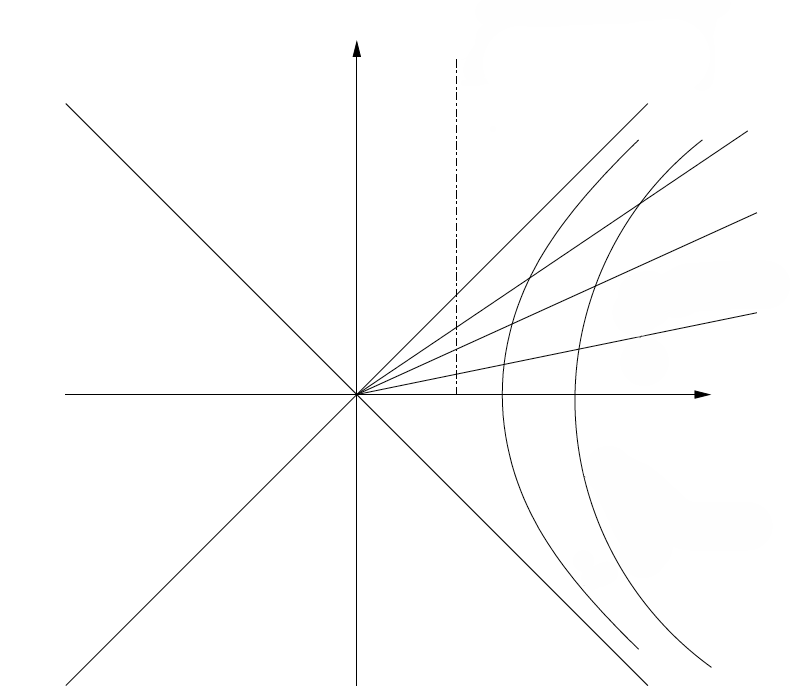
\includegraphics[width=6cm]{../img/rindler-space.png}
\caption{Here are shown all possible hyperbolic trajectories with $a>0$. The vertical straight line is the world line of a stationary observer.}
\end{figure}

Notice that choosing negative acceleration $a<0$ trajectories are in the left side of the space, i.e. trajectories for positive and negative acceleration lives in disconnected regions. 

For $\tau=0$ we have $u^0(\tau=0)=\cosh(0)=1$ and $u^1(\tau=0)=\sinh(0)=0$, i.e. we are in the rest frame for our system. Since $X$ is the value of $x$ for $\tau=0$, then $X$ can be interpreted as the proper $x$ coordinate for a particle accelerating on the $x$ direction (analogously as $\tau$ for the time). Equivalently, let $\de X$ be the infinitesimal distance between two close coordinates for the system in the rest frame, then $\de x$ for $\tau\neq0$ is the contracted distance between the two coordinates when the system has non-zero velocity:
\[\de x=\frac{\de X}\gamma\]
\begin{figure}[H]
\centering
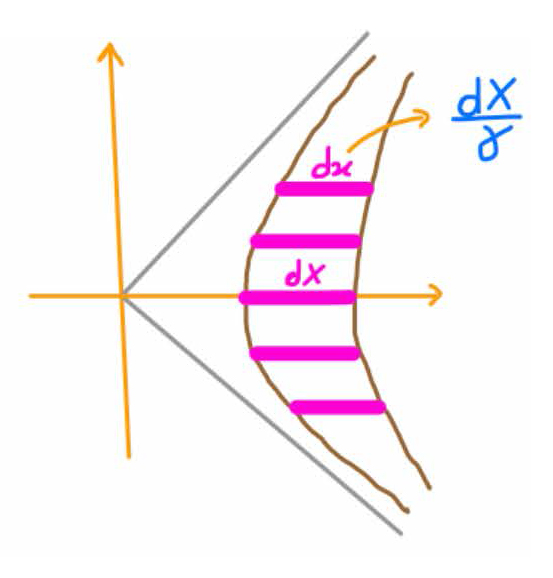
\includegraphics[width=4cm]{../img/X-proper-lenght-Rindler.jpg}
\end{figure}
Let's prove the last statement. For $t=$const., we have $\de t=[\sinh(\tau/X)\de X+\cosh(\tau/X)\de\tau]=0$ and this means
\[\de\tau=-\tanh(\frac\tau X)\de X\]
then we have
\[\de x=\cosh(\frac\tau X)\de X+\sinh(\frac\tau X)\de\tau=\frac1{\cosh(\tau/X)}\de X=\frac{\de X}\gamma\]

Therefore the family of hyperbolic trajectories describes motion of points of a rigid body accelerating on the $x$ direction. 

Notice that accelerations of points on the rigid body are all different, since different points belong to different trajectories, i.e. corresponds to different values for $a$. In our one-space-dimensional model this means that all points of the rod in the following picture has different acceleration\footnote{This can also be interpreted as the origin of the contraction of lengths.}:
\begin{figure}[H]
\centering
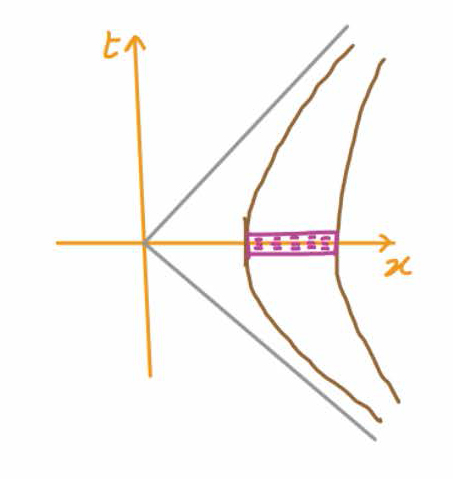
\includegraphics[width=4cm]{../img/acceleration-points-rigid-body.jpg}
\end{figure}
This is not true for higher dimensions since all points in a hyperplane orthogonal to the direction of motion have same acceleration. Anyhow points on different hyperplanes must have different accelerations.

Notice also that quantity $x^2-t^2=X^2$ is invariant under Lorentz transformation (i.e. 4-dimensional rotations), and then going from an inertial frame into another we have the same equation $\tilde x^2-\tilde t^2=X^2$. In particular for any inertial frame when $\tilde t=0$ all points of the rod are at rest and $\Delta \tilde x(\tilde t=0)=\Delta X$, i.e. all distances are equivalent in all rest frames. 
\begin{figure}[H]
\centering
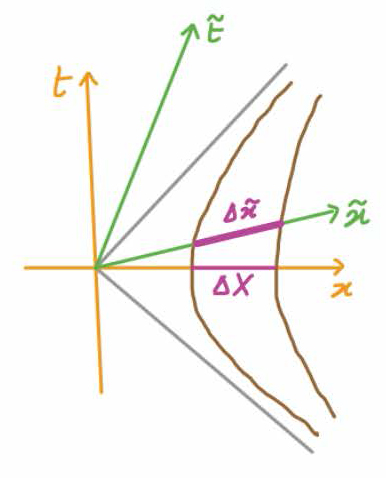
\includegraphics[width=4cm]{../img/equivalence-rest-frames.jpg}
\end{figure}

Using last observation, we can think about $X$ as a coordinate for (instead of a rod) a rigid lattice, parametrized by space coordinates $X$, $Y$, $Z$, where $Y=y$ and $Z=z$ are usual Euclidean coordinates. We consider only the connected lattice defined by $X>0$ (i.e. $a>0$).
So far we used to parametrize each trajectory with its proper time $\tau$ measured by a clock moving on the trajectory. Therefore we can use as coordinate system of our lattice the set $(\tau,X,Y,Z)$. 

In order to describe what is special with this reference frame, let's consider line elements:
\[\begin{cases}
x^0=X\sinh(\frac\tau X)\\
x^1=X\cosh(\frac\tau X)
\end{cases}
\qquad\Rightarrow\qquad
\begin{cases}
\de x^0=\left[\sinh(\tau/X)-\frac\tau X\cosh(\frac\tau X)\right]\de X+\cosh(\frac\tau X)\de\tau\\
\de x^1=\left[\cosh(\tau/X)-\frac\tau X\sinh(\frac\tau X)\right]\de X+\sinh(\frac\tau X)\de\tau
\end{cases}\]
and then the metric reads
\begin{align}\label{eqn:Rindler-metric-tau}
\de s^2&=\eta_{\mu\nu}\de x^\mu\de x^\nu\\
&=-\de\tau^2+\frac{2\tau}{X}\de\tau\,\de X+\p{1-\frac{\tau^2}{X^2}}\de X^2+\de Y^2+\de Z^2
\end{align}
This non-trivial metric can be regarded as fully characterising the new frame, so is telling us how coordinates (identified as position on the lattice and proper time measured by accelerating clocks) enter into the definition of line elements. 

So far we could simply think about this metric as the consequence of a simply change of coordinates, and not really matter. But now invoking the equivalence principle, we can say that the accelerated frame described by coordinates  $(\tau,X,Y,Z)$ should be equivalent to a frame undergoing gravitational force.
Therefore the existence of gravitational field could be revisited as the existence of a non trivial metric in our spacetime. 


\section{The Rindler spacetime}
\textbf{Blau sec. 1.3; 't Hooft chap. 3}\\

 In the previous section we constructed the rigid lattice with coordinates $(\tau,X,Y,Z)$ and non-trivial metric\footnote{Usually in these notes terms ``metric" and ``line element" are used equivalently, beside in the formal definition of metric that we will introduce in the next chapters.} \eqref{eqn:Rindler-metric-tau} where $\tau$ and $X$ are respectively proper time and proper length in this lattice. 
Note that the components of the metric depend on $(\tau,X)$. In particular, the separation between simultaneous events $A$ and $B$ (with $\tau_A=\tau_B$) is not the Eucledian one ($\Delta l^2=\Delta X^2+\Delta Y^2+\Delta Z^2$) and changes with time $\tau$.

Despite the physical meaning of $\tau$ as proper time, a nicer coordinate $T$ can be chosen for lattice's system of coordinates. Note that
\[\de s^2=-\p{\de\tau-\frac\tau X\de X}^2+\de X^2+\de Y^2+\de Z^2\]
therefore if we define following \emph{adimensional} coordinate
\[T=\frac\tau X\]
and we use it instead of $\tau$, following substitutions must be done
\[\tau=XT\qquad\Rightarrow\qquad\de\tau=X\de T+T\de X=X\de T+\frac\tau X\de X\]
 and the line element takes the form
\begin{equation}\label{eqn:Rindler-metric}
\de s^2=-X^2\de T^2+\de X^2+\de Y^2+\de Z^2
\end{equation}

The spacetime equipped with metric eq.\eqref{eqn:Rindler-metric} is called \textbf{Rindler spacetime}. 
Notice that same metric can be obtained directly from the flat spacetime using following substitutions
\[\begin{cases}
t=X\sinh T\\
x=X\cosh T
\end{cases}\]

\subsubsection{Proprieties of the coordinates system of Rindler space}

One of main advantages of the system of coordinates $(T,X,Y,Z)$ is that if we consider simultaneous events ($\de\tau=0=\de T$) then metric eq.\eqref{eqn:Rindler-metric} is the Euclidean one. Also, if we draw the Rindler space as follows:
\begin{figure}[H]
\centering
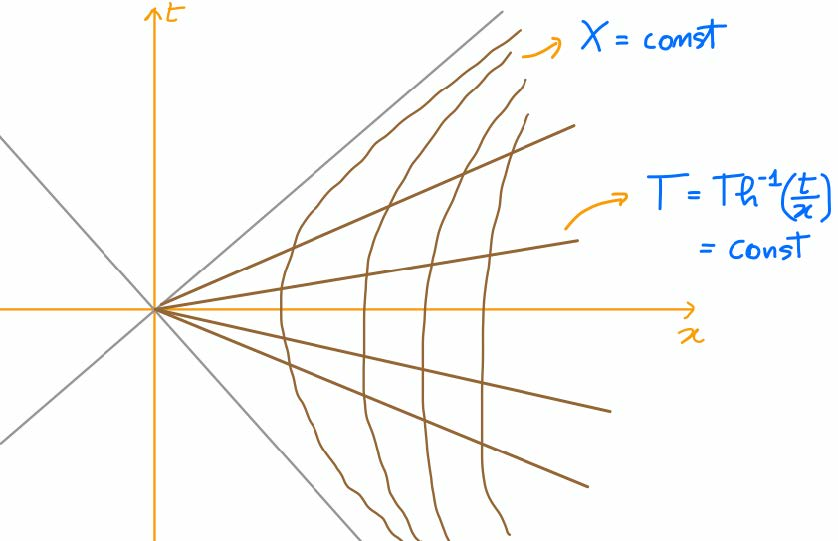
\includegraphics[width=7cm]{../img/rindler-space2.jpg}
\end{figure}
\noindent then points with constant $X$ corresponds to hyperbolic trajectories with constant acceleration, and points with constant $T$ are placed on the same straight line passing through the origin, in particular proper time is given by the relation
\[T=\tanh^{-1}\p{\frac tx}\]

Moreover, suppose that two clocks moving with constant acceleration are placed on the lattice, and one of them (namely ``clock $A$'') sends light signals to the other (called ``clock $B$''). Let $T_A$ be the proper time for $A$ when the first clock sends the signal and $T_B$ be the proper time for $T_B$ when the second clock receives the signal. Then the difference $\Delta T=T_B-T_A$ does not depend on the time when the first clock sends it signal, i.e. $\Delta T$ is time-independent: if clock $A$ send another light signal at the proper time $T_A'$, which is received by the clock $B$ at proper time $T_B'$, then $T_B-T_A=T_B'-T_A'$.
\begin{figure}[H]
\centering
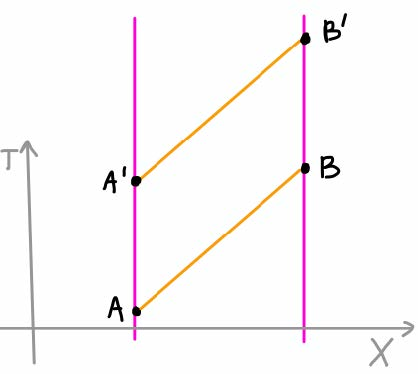
\includegraphics[width=4.5cm]{../img/T-meaning-Rindler.jpg}
\end{figure}
\noindent In other words, if $A$ sends light signals with a certain rate, then the clock $B$ ``sees''\footnote{``Sees'' mean seen by light signals.} clock $A$ ``clicking'' with the same rate. We can prove this as follows: first of all for the light signal we have $\de s^2=0$, then
\[0=\de s^2=-X^2\de T^2+\de X^2\qquad\Rightarrow\qquad\de T=\frac{\de X}{X}\]
where in the second step we fixed the sign in order to choose the right direction of propagation (shown in the picture). If we consider the value of $\Delta T\equiv T_B-T_A$, i.e. the time between the click of $A$ and the light signal seen by $B$, we have
\[\Delta T\equiv T_B-T_A=\int_A^B\de T=\int_A^B\frac{\de X}{X}=\log\frac{X_B}{X_A}\] 
this means that $\Delta T$ depends only on the proper position on the lattice of the two clocks, hence does not depend on the time $T_A$ when the first clock clicks:
\begin{align*}
T_B&=T_A+\Delta T\\
T_{B'}&=T_{A'}+\Delta T
\end{align*}
We can also say that using time coordinate $T$ then times of clocks are syncronized by light signals.
This propriety is called propriety of \textbf{static} spacetime. 

We seen that give EEP implies that this accelerating frame (the Rindler space) could be interpreted as a frame undergoing a gravitational field. This leads a non-trivial acceleration of free-falling objects. We know that acceleration experienced by points in the lattice is given by $\vec a=-(1/X)\hat u_x$, then just applying EEP we can obtain the formula for the gravitational field: 
\[\vec a_G=-(1/X)\hat u_x=-\vect\nabla\Phi\qquad\Rightarrow\qquad\Phi=\log X\]
Notice that in this realization of EEP the gravitational field is not constant, since its strength is proportional to $-\vect\nabla\Phi$ and then decreases with $X$ (in particular, respect to the last picture, the field strength is weaker in $B$ than in $A$). Using $\Phi=\log X$ we can rewrite Rindler metric in the following form
\begin{equation}\boxed{
\de s^2=-e^{2\Phi}\de T^2+\de X^2+\de Y^2+\de Z^2
}\end{equation}
where basically respect to the flat metric we changed the coefficient of the time component by a factor given by the gravitational potential. This confirms our suggestion\footnote{By the analogy with EM we were looking for a way to rewrite gravitational laws in relativistic way using gravitational potential.}, namely by applying equivalence principle the potential associated to a specific gravitational field can be identified as a part of the metric specifying the frame in which the object experience such gravitational field. 
This will lead us to treat and complete the notion of gravitational potential with the metric itself characterizing a given spacetime. 

Before starting to work on the complete theory of GR, let's consider other proprieties of Rindler space. 
Now we will discuss how Rindler spacetime already exhibits some effects that we will encounter in more general settings. 

\subsubsection{Time dilatation and red-shift}

In previous sections we described time dilatation and red-shift using non-relativistic arguments, now we will analyze them using relativistic treatment.
Consider again next picture:
\begin{figure}[H]
\centering
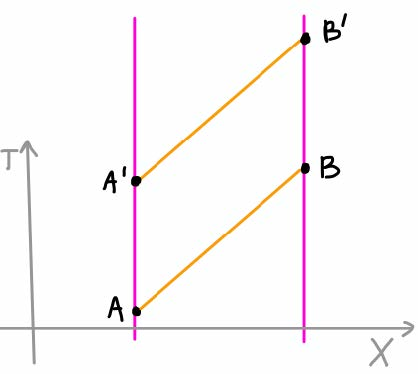
\includegraphics[width=4.5cm]{../img/T-meaning-Rindler.jpg}
\end{figure}
\noindent we know that the proper time is related with $T$ by the relation $\tau=XT$. This means that the proper time interval between events $B$ and $B'$ can be written as follows
\[\tau_{B'}-\tau_B=X_B(T_{B'}-T_B)=X_B(T_{A'}-T_A)=\frac{X_B}{X_A}(\tau_{A'}-\tau_A)\]
and using gravitational potential we have:
\[\boxed{
\Delta\tau_B=\frac{X_B}{X_A}\Delta\tau_A=e^{\Phi_B-\Phi_A}\Delta\tau_A
}\]
If instead of clocks synchronized by light signals (i.e. measuring the value $T$) we consider 2 identical clocks measuring the proper time, then they ``see'' each other running differently:
\begin{enumerate}[label=\textbullet]
\item clock $B$ ``sees'' clock $A$ going \emph{slower} by factor $X_A/X_B=e^{\Phi_A-\Phi_B}<1$
\item clock $A$ ``sees'' clock $B$ going \emph{faster} by factor $X_B/X_A=e^{\Phi_B-\Phi_A}>1$
\end{enumerate}
Let's see this effect in terms of frequencies. If $\Delta\tau=1/\nu$ then we have
\[\nu_B=\frac{X_A}{X_B}\nu_A\qquad\Rightarrow\qquad\nu_B<\nu_A\]
and then this shows \emph{red-shift effect}. If $X_B=X_A+\delta X$ for $\delta X\ll1$ then gravitational potential can be thought as linear and
\[\frac{\nu_B-\nu_A}{\nu_A}=\p{\frac{X_A}{X_B}-1}\simeq-\frac{\delta X}{X_A}=-\delta\Phi\simeq-\frac{1}{c^2}(\Phi_B-\Phi_A)\]
where in the last step we restored the constant $c$.
Energy of photons is proportional to them frequency ($E=h\nu$) so the difference between energy in $A$ and energy $B$ can be seen as the energy lost by the photon due to the fact that it is ``climbing'' the potential $\Phi$ (i.e. difference of energy is related to the difference of potential energy between $A$ and $B$).

\subsubsection{Event horizons}
A second propriety of Rindler space is related to the presence of \textbf{event horizons}. Similar phenomena will appear in the treatment of black holes, but Rindler space can be used as toy model for it description and understanding. First observation is that $X$ Rindler's coordinate is restricted to be positive, and we can see that the metric became degenerate for $X=0$:
\[\de s^2=-X^2\de T^2+\de X^2+\de Y^2+\de Z^2\]
i.e. we have a coordinate singularity for $X=0$. In particular for $X=0$ a purely time like difference $\Delta T$ between two events happening at different times becomes light-like. However, recovering original flat metric in a inertial frame (in particular we do not restrict only to the  $X>0$ case), then this metric is equivalent to a smooth metric well defined. The singularity is due to our specific choice of coordinates, and is not related to the geometry of the space itself.\footnote{In Differential Geometry terminology, this means that our chart is well defined only on the open set corresponding to $X>0$ local coordinates. On the other hand, we can find different charts and an atlas that covers all the $\RR^4$ space with well defined coordinates for each point. For example, the Minkowski system of coordinates defines an atlas well defined on all the space. Rindler system of coordinates is just a system of coordinates comfortable for our description of trajectories when $X>0$. This won't be true for singularities in black holes.} This somehow correspond to the $r=0$ case for radial coordinates $\de r^2+r^2\de\theta^2$: the flat space has its own well defined, smooth, metric, but with a specific choice of coordinates we could obtain a degenerate metric in some point, like the origin for radial coordinates or $X=0$ for the Rindler space. 

On the other hand the point corresponding to $X=0$ has some special proprieties: recall $X\equiv\sqrt{x^2-t^2}$, then $X=0$ is the interception of two lines: $x=\pm t$. These two lines can be interpreted as horizons of Rindler spacetime, they separate Rindler space time to the remaining of the full Minkowskian spacetime:
\begin{figure}[H]
\centering
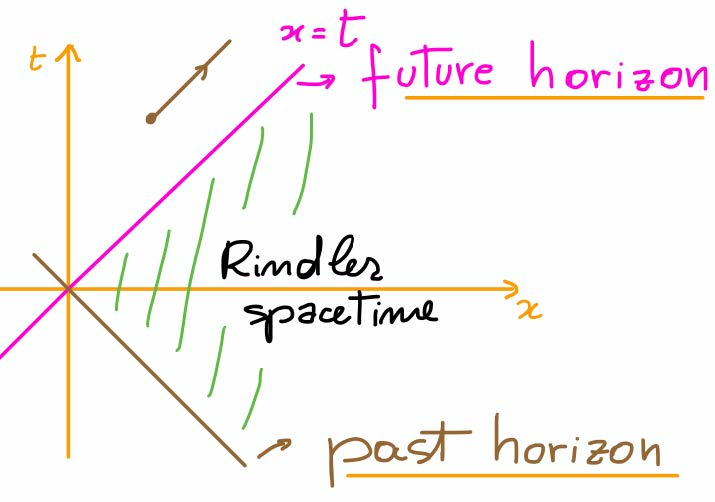
\includegraphics[width=5.5cm]{../img/rindler-horizons.jpg}
\end{figure}
\noindent In particular, the right side of $x=t$ horizon is the boundary between events in the Rindler spacetime and events that cannot be reached by Rindler events. In other word, Rindler events cannot ``see'' beyond the future horizon line, i.e. events above the future horizon line cannot send signal to Rindler space. In the opposite, right side of the past horizon straight line represents the boundary between Rindler space and events that cannot receive any signal from Rindler space. 

As we will see horizon will emerge in more general models and will actually characterize black holes.

Any observer freely ``falling''\footnote{This means that he can freely move in Minkowski space.} towards the horizon will cross it in a finite proper time (recall that $t$ is the proper time if the observer is at rest), as it is pictorially represented in the next picture.
\begin{figure}[H]
\centering
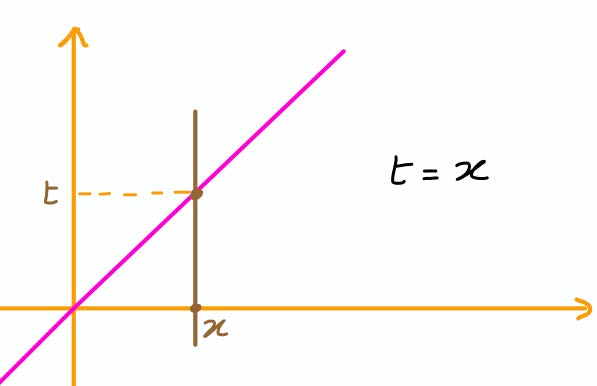
\includegraphics[width=5cm]{../img/observer-crossing-horizon-prop-time.jpg}
\end{figure}
\noindent If, instead of measuring time using proper time, we use the coordinate $T$, then we know that $\tanh T_A=t_a/x_a$ and therefore when the observer cross the horizon we have $\tanh T_A=1$, which implies that $T_A=\infty$. This means that if we try to describe a freely ``falling'' observer using Rindler coordinates, it can reach the horizon in a finite time, but then it needs an infinite amount of time in order to cross the boundary.
If we suppose that, referencing to the next figure, an observer placed in $A$ sends with a certain proper period a light signal to a Rindler observer (i.e. that movers with constant acceleration) placed in B and the latter measure the rate between signals, we can see that when $A$ is crossing the horizon
\[\Delta \tau_B=X_B\Delta T_B=X_B\Delta T_A=\infty\]
\begin{figure}[H]
\centering
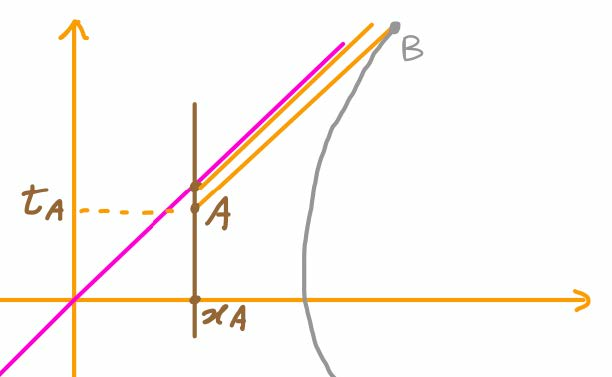
\includegraphics[width=5cm]{../img/observer-crossing-horizon-T-time.jpg}
\end{figure}
\noindent This means that even though the first observer cross the horizon in a finite proper time, the observer B never ``sees'' the first observer crossing the horizon. This can be also understood by observing that the light signal when $A$ approaches the horizon will take more and more time to reach B and in particular when A is crossing the horizon then the light signal will take an infinite time $T$ to reach B.


\section{From the Equivalence Principle to curved spacetime}
Up to now we have seen that the EEP leads us to associate a gravitational field to a non-trivial metric. On the other hand the discussion leads us to the idea that the Rindler gravitational field may be considered ``fake'': we can make a global change into free-falling/inertial coordinates. In this way, we can also treat orther example of fake gravitational fields, that can be associated to other non-trivial metric in some more general coordinates $X^\mu$:
\begin{equation}\label{eqn:non-trivial-metric-fake-field}
g_{\mu\nu}(X)=\eta_{\rho\sigma}\frac{\partial x^\rho}{\partial X^\mu}\frac{\partial x^\sigma}{\partial X^\nu}
\end{equation}
so that  the line element takes the form
\[\de s^2=\eta_{\mu\nu}\de x^\mu \de x^\nu=g_{\mu\nu}(X)\de X^\mu\de X^\nu\]

Vice versa, we can say that the gravitational field associated to some metric $g_{\mu\nu}$ is ``fake'' if we can find a global ``freely-falling'' frame $x^\mu(X)$ such that \eqref {eqn:non-trivial-metric-fake-field} holds. 
\footnote{An interesting example is given by an uniformly rotating frame in Minkowski space, described in \textsf{Rindler sec. 9.7}}

One can then consider more general metrics $g_{\mu\nu}(x)$ such that  \eqref {eqn:non-trivial-metric-fake-field} does not hold. In such a case the metric can be identified with the ``\emph{genuine}'' gravitational potetial, i.e. a potential that cannot be interpreted as a ``freely-falling'' frame. 
In analogy to the EM potential one can think of the ``fake'' gravitational potential as a vector potential which is a pure gauge potential (i.e. can be written as derivative of some function defining gauge transformation), while a ``genuine'' gravitational potential would correspond to a gauge field associated to a non trivial field strength.

We then need to study general metrics $g_{\mu\nu}(x)$ in general coordinate systems, and in order to do this we must consider more general space-times. For example we will consider the gravitational field produced by a spherical object

\begin{figure}[H]
\centering
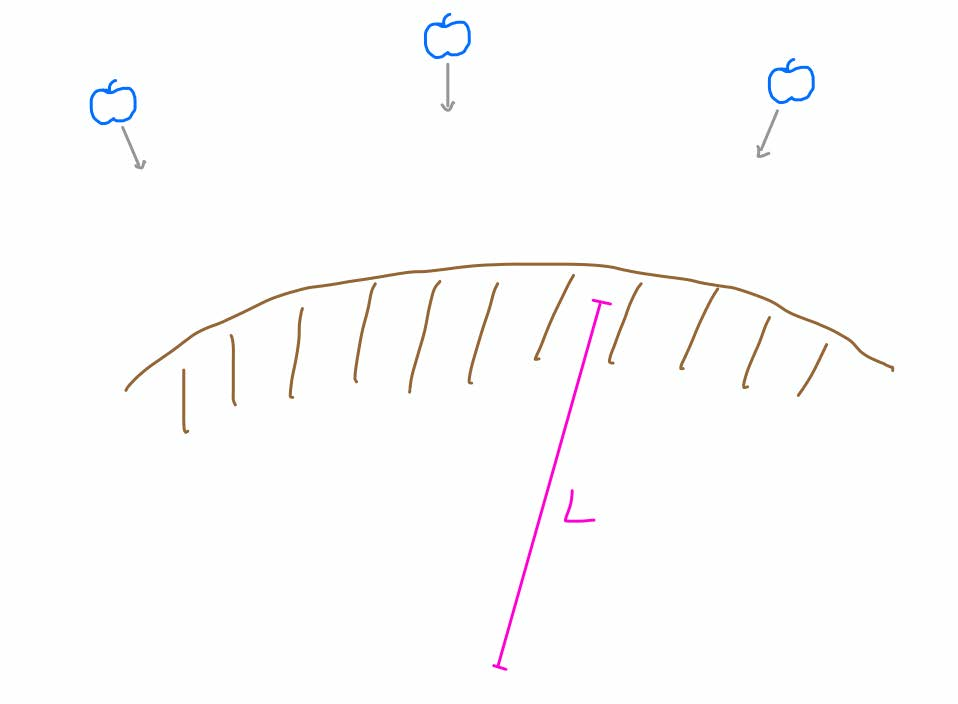
\includegraphics[width=5cm]{../img/grav-field-spheric-apples.jpg}
\end{figure}

\noindent This is a (very important) example of a ``genuine'' gravitational potential. There is no way to define a global ``freely falling'' reference frame, this is possible only in a small neighbourhood of the object we would like to consider, where the potential is considered linear.

Recall our statement of EEP: ``\emph{In a small enough region of the space-time, the laws of physics reduce to those of SR}'', this means that only in small regions of space-time we can go into ``freely-falling'' frames where the physics reduces to SR one. 
It translates into the existence of local frames, i.e. space-time coordinates $x^\mu$ in which 
\[g_{\mu\nu}(x)\simeq \eta_{\mu\nu}+o\p{\frac{x^2}{L^2}}\]
so in a certain sense the typical length scales $L$ ``measure'' how ``honest'' the gravitational field is, which is associated to the Tidal effect; $L$ also parametrize the deviation from Minkowski spacetime, and in other words we will see that this corresponds to the curvature of the space-time. 

We need a mathematical language in which
\begin{enumerate}[label=\textbullet]
\item there is no preferred globally defined coordinate system / frame $x^\mu$ (the inertial frames are not preferred respect to the others, they are just the coordinate system where the Minkowski metric is the flat one)
\item intervals defined by a metric $g_{\mu\nu}(x)$ are associated to line elements in the form
\[\de s^2=g_{\mu\nu}(x)\de x^\mu\de x^\nu\]
\item $g_{\mu\nu}(x)$ is the (\emph{dynamical}) gravitational field
\item the equation that describe the space time must be coordinate independent, i.e. we require a general covariance of physical laws
\end{enumerate}
Notice also that in order to satisfy these requirements the global spacetime need no to be same of $\text{Mink}^4\simeq\RR^4$, but it will be determined by dynamics, i.e. from $g_{\mu\nu}(x)$. 
Differential geometry provides the natural mathematical framework/language to formulate such a theory.  

















\end{document}